\documentclass[12pt, oneside]{article}
\usepackage[letterpaper, margin=1in, headsep=0.5in]{geometry}
\usepackage[english]{babel}
\usepackage[utf8]{inputenc}
\usepackage{amsmath}
\usepackage{amsfonts}
\usepackage{amssymb}
\usepackage{tikz}
\usetikzlibrary{quotes, angles}
\usepackage{graphicx}
%\usepackage{pgfplots}
%\pgfplotsset{width=10cm,compat=1.9}
%\usepgfplotslibrary{statistics}
%\usepackage{pgfplotstable}
%\usepackage{tkz-fct}
%\usepackage{venndiagram}

\usepackage{fancyhdr}
\pagestyle{fancy}
\fancyhf{}
\rhead{\thepage \\Name: \hspace{1.5in}.\\}
\lhead{BECA / Dr. Huson / 10th Grade Geometry\\* 25 October 2018}

\renewcommand{\headrulewidth}{0pt}

\begin{document}
\subsubsection*{Do Now: Midpoint and distance review}
Show your work. For graphs, use a pencil and straight edge.
  \begin{enumerate}

%\subsubsection*{Use the graph and the midpoint formula}
\item Given $A(-2, 5)$ and $B(4, 1)$.
\begin{enumerate}
  \item Plot and label the points on the graph, drawing $\overline{AB}$
  \item Write down the midpoint formula, substituting coordinate values.
  \item Find the midpoint's coordinates.
  \item Plot and label the midpoint, $M$, on the graph.
\end{enumerate}}

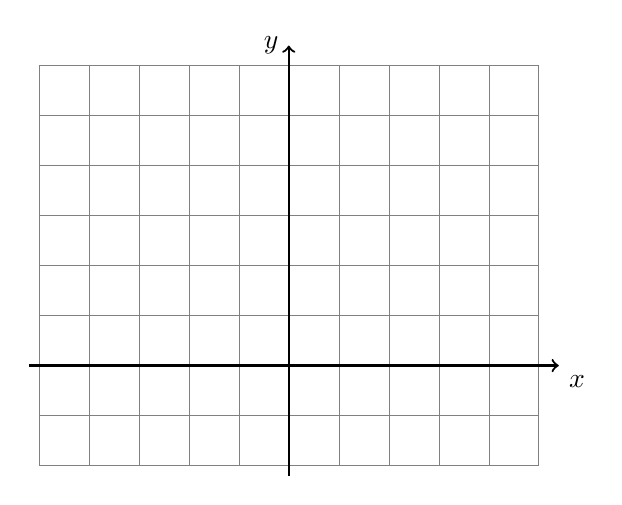
\begin{tikzpicture}[scale=.635]
  \draw [help lines] (-5,-2) grid (5,6);
  \draw [thick, ->] (-5.2,0) -- (5.4,0) node [below right] {$x$};
  \draw [thick, ->] (0,-2.2)--(0,6.4) node [left] {$y$};
\end{tikzpicture}

%\subsubsection*{The Pythagorean formula and distance on the plane}
\item Given $C(-4, -3)$, $D(2, 5)$, and $E(2, -3)$.
\begin{enumerate}
  \item Plot and label the points on the graph, drawing $\overline{CD}$
  \item Draw the legs of the right triangle, $\overline{CE}$ and $\overline{ED}$, marking their lengths.
  \item Write down the distance formula for $CD$, substituting coordinate values.
  \item Find the value of $CD$.
\end{enumerate}}

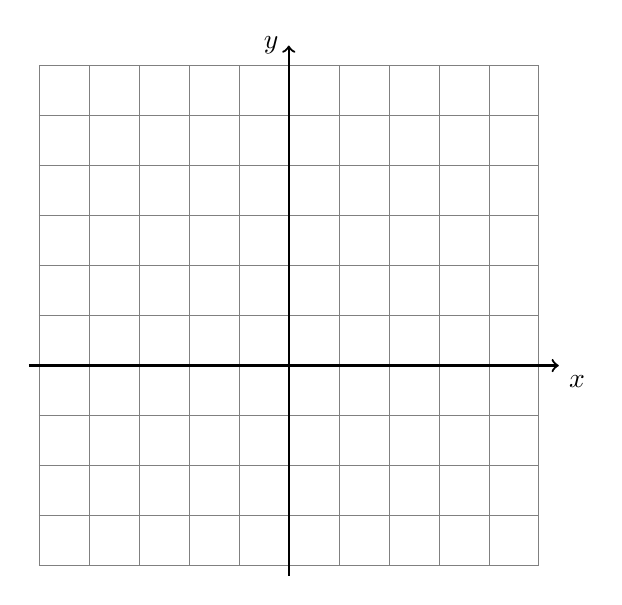
\begin{tikzpicture}[scale=.635]
  \draw [help lines] (-5,-4) grid (5,6);
  \draw [thick, ->] (-5.2,0) -- (5.4,0) node [below right] {$x$};
  \draw [thick, ->] (0,-4.2)--(0,6.4) node [left] {$y$};
\end{tikzpicture}

\end{enumerate}
\end{document}
